\section{Saltos}

\begin{frame}[fragile]{Saltos}

    \begin{itemize}
        \item As atribuições simulam as instruções de escrever ou apagar um traço nas fitas das
            máquinas de Turing

        \item Assim, as linguagens imperativas precisam também de mecanismos que permitam que o
            controle decida o próximo estado a ser avaliado de forma condicional, de acordo com o
            estado atual

        \item Nas linguagens Assembly isto é feito por meio de saltos condicionais

        \item Os saltos são instruções que desviam o controle para pontos específicos, 
            identificados por rótulos, de acordo com o estado dos registradores de controles
            ({\it flags})

        \item Como podem existir diversas combinações das (\textit{flags}) a serem
            consideradas, há várias instruções de salto distintas

        \item Também existe uma instrução para saltos incondicionais
    \end{itemize}

\end{frame}

\begin{frame}[fragile]{Salto incondicional}

    \begin{itemize}
        \item A instrução \code{nasm}{JMP} corresponde a um salto incondicional

        \item A sintaxe desta instrução é

            \inputsyntax{nasm}{codes/jmp.st}

        \item \textit{label} corresponde a um rótulo, e a execução do programa seguirá para a
            primeira instrução que segue o rótulo

        \item Como o salto é incondicional, a depender do posicionamento da instrução de salto e
            do rótulo o programa pode ficar preso em um laço infinito, jamais encerrando sua
            execução

        \item Ainda assim, saltos incondicionais são úteis, principalmente para sair de laços 
            aninhados ou para encerrar o programa a partir de qualquer ponto
    \end{itemize}

\end{frame}

\begin{frame}[fragile]{Saltos condicionais}

    \begin{itemize}
        \item Um salto condicional avalia uma ou mais \textit{flags} e, a depender dos estados
            delas (0 ou 1), realiza o salto ou não

        \item A instrução \code{nasm}{JZ} salta para \textit{label} se a \textit{flag} zero for 
            igual a 1

        \item As instruções \code{nasm}{ADD} e  \code{nasm}{SUB} modificam esta \textit{flag}, 
            tornando igual a 1 se o resultado da operação é igual a zero, ou 0, caso contrário

        \item A instrução \code{nasm}{JNZ} salta para \textit{label} se a \textit{flag} zero for 
            igual a 0

        \item Outra \textit{flag} que é modificada pelas instruções \code{nasm}{ADD} e 
            \code{nasm}{SUB} é a de sinal, que se torna um se o resultado da operação é negativo,
            ou zero, caso contrário

        \item As instruções \code{nasm}{JS} e \code{nasm}{JNS} são semelhantes às instruções
            \code{nasm}{JZ} e \code{nasm}{JNZ}, porém elas avaliam a \textit{flag} de sinal
    \end{itemize}

\end{frame}

\begin{frame}[fragile]{Exemplo de saltos condicionais}
    \inputsnippet{nasm}{1}{22}{codes/roots.s}
\end{frame}

\begin{frame}[fragile]{Exemplo de saltos condicionais}
    \inputsnippet{nasm}{23}{43}{codes/roots.s}
\end{frame}

\begin{frame}[fragile]{Exemplo de saltos condicionais}
    \inputsnippet{nasm}{44}{66}{codes/roots.s}
\end{frame}

\begin{frame}[fragile]{Comparações}

    \begin{itemize}
        \item Outra \textit{flag} que é modificada pelas operações aritméticas é a de 
            \textit{overflow}

        \item As diferentes combinações das \textit{flags} de sinal, de \textit{overflow} e zero
            permite simular os operadores relacionais das linguagens de programação de 
            alto nível

        \item A instrução \code{nasm}{CMP}, cuja sintaxe é

            \inputsyntax{nasm}{codes/cmp.st}

        compara o conteúdo dos registradores \texttt{x} e \texttt{y}, modificando as \textit{flags}
        apropriadas

        \item Após esta instrução, é possível utilizar um dos comandos de saltos listados na
            tabela a seguir

        \item Observe que há um conjunto de instruções para inteiros sinalizados e outro para
            inteiros não sinalizados

        \item Veja que, se após a instrução \code{nasm}{CMP} e antes do salto, for executada
            alguma instrução que modifique alguma das \textit{flags}, o salto pode não ter o
            efeito esperado

    \end{itemize}

\end{frame}

\begin{frame}[fragile]{Saltos associados aos operadores relacionais}

    \begin{table}[ht]
        \centering
        \begin{tabular}{ccl}
            \toprule
            \textbf{Sinalizados} & \textbf{Não sinalizados} & \textbf{Efeito} \\
            \midrule
                \texttt{JL} & \texttt{JB} & Salta se $x < y$ \\
                \texttt{JLE} & \texttt{JBE} & Salta se $x \leq y$ \\
                \texttt{JG} & \texttt{JA} & Salta se $x > y$ \\
                \texttt{JGE} & \texttt{JAE} & Salta se $x \geq y$ \\
                \texttt{JE} & \texttt{JE} & Salta se $x = y$ \\
            \midrule
                \texttt{JNL} & \texttt{JNB} & Salta se $x \nless y$ \\
                \texttt{JNLE} & \texttt{JNBE} & Salta se $x \nleq y$ \\
                \texttt{JNG} & \texttt{JNA} & Salta se $x \ngtr y$ \\
                \texttt{JNGE} & \texttt{JNAE} & Salta se $x \ngeq y$ \\
                \texttt{JNE} & \texttt{JNE} & Salta se $x \neq y$ \\
            \bottomrule
        \end{tabular}
        
    \end{table}

    \vspace{0.2in}

    \textbf{Observação}: \texttt{L} = \textit{less}, \texttt{G} = \textit{greater}, 
        \texttt{A} = \textit{above}, \texttt{B} = \textit{below}, \texttt{J} = \textit{jump}, 
        \texttt{E} = \textit{equal}, \texttt{N} = \textit{not} 

\end{frame}

\begin{frame}[fragile]{Exemplo de comparações}
    \inputsnippet{nasm}{1}{21}{codes/parity.s}
\end{frame}

\begin{frame}[fragile]{Exemplo de comparações}
    \inputsnippet{nasm}{22}{45}{codes/parity.s}
\end{frame}

\begin{frame}[fragile]{\tt IF-ELSE}

    \begin{itemize}
        \item Os saltos condicionais permitem simular estruturas de controle presentes em outras
            linguagens

        \item O construto \texttt{IF-ELSE} tem a seguinte sintaxe:

            \inputsyntax{haskell}{codes/if_else.st}

        \item Se a \texttt{condicao} for avaliada como verdadeira, são executados os comandos
            associados ao \texttt{blocoA}; caso contrário, são executados os comandos do
            \texttt{blocoB}

        \item A cláusula \texttt{ELSE} é opcional

        \item Este construto desvia a execução do programa, que a partir da condição passa a
            ter dois caminhos possíveis, e estes caminhos são mutuamente exclusivos

        \item Após o término do bloco escolhido, a execução continua do ponto que segue o último
            comando associado a \texttt{blocoB}
    \end{itemize}

\end{frame}

\begin{frame}[fragile]{Visualização do construto {\tt IF-ELSE}}
    \begin{figure}[ht]
        \centering
        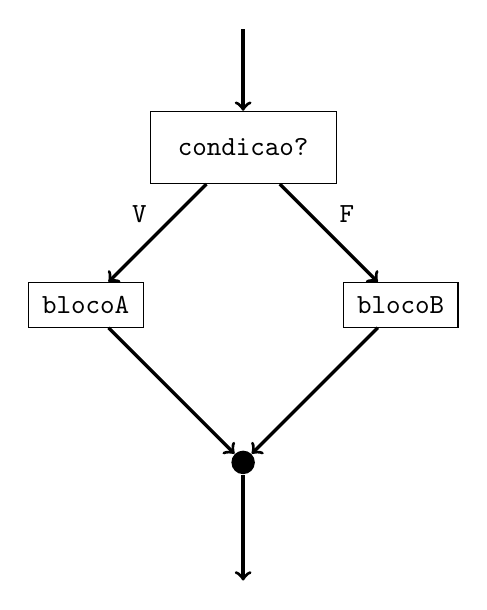
\begin{tikzpicture}
            \coordinate (A) at (0, 1.5);
            \coordinate (B) at (0, -4);
            \coordinate (C) at (0, -5.5);

            \node[draw,inner sep=10pt] (IF) at (0, 0) { \tt condicao? };
            \node[draw,inner sep=5pt] (BA) at (-2, -2) { \tt blocoA };
            \node[draw,inner sep=5pt] (BB) at (2, -2) { \tt blocoB };
            \node[fill,circle,inner sep=3pt] (RESUME) at (B) { };

            \draw[->,very thick] (A) -- (IF);
            \draw[->,very thick] (IF) -- node[anchor=south east] { \tt V } (BA);
            \draw[->,very thick] (IF) -- node[anchor=south west] { \tt F } (BB);
            \draw[->,very thick] (BA) -- (RESUME);
            \draw[->,very thick] (BB) -- (RESUME);
            \draw[->,very thick] (RESUME) -- (C);

        \end{tikzpicture}
    \end{figure}
\end{frame}

\begin{frame}[fragile]{Codificação do construto {\tt IF-ELSE} em Assembly}
    \inputsnippet{nasm}{1}{22}{codes/if.s}
\end{frame}

\begin{frame}[fragile]{\tt WHILE}

    \begin{itemize}
        \item Outro construto que pode ser simulado com saltos condicionais é o laço \texttt{WHILE}

        \item A sintaxe do laço \texttt{WHILE} é

            \inputsyntax{pascal}{codes/while.st}

        \item Os comandos associados ao \texttt{bloco} serão executados sempre que a 
            \texttt{condicao} for verdadeira

        \item Deste modo, caso os comandos do bloco não alterem o estado do programa de modo 
            a permitir que a condição se torne falsa, o laço se repetirá indefinidamente

        \item A presença de saltos dentre os comandos do bloco permite a saída prematura do bloco
    \end{itemize}

\end{frame}

\begin{frame}[fragile]{Visualização do construto {\tt WHILE}}
    \begin{figure}[ht]
        \centering
        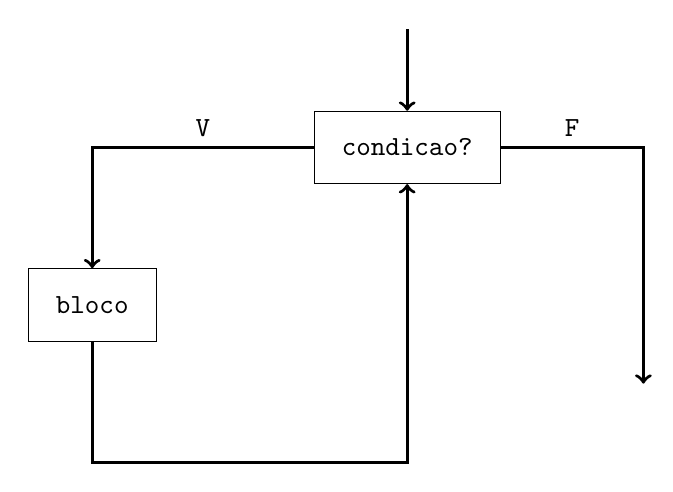
\begin{tikzpicture}
            \coordinate (A) at (0, 1.5);
            \coordinate (B) at (-4, 0);
            \coordinate (C) at (-4, -4);
            \coordinate (D) at (0, -4);
            \coordinate (E) at (3, 0);
            \coordinate (F) at (3, -3);

            \node[draw,inner sep=10pt] (WHILE) at (0, 0) { \tt condicao? };
            \node[draw,inner sep=10pt] (BA) at (-4, -2) { \tt bloco };

            \draw[->,very thick] (A) -- (WHILE);
            \draw[->,very thick] (WHILE) -- node[anchor=south] { \tt V } (B) -- (BA);
            \draw[->,very thick] (BA) -- (C) -- (D) -- (WHILE);
            \draw[->,very thick] (WHILE) -- node[anchor=south] { \tt F } (E) -- (F);

        \end{tikzpicture}
    \end{figure}
\end{frame}

\begin{frame}[fragile]{Codificação do construto {\tt WHILE} em Assembly}
    \inputsnippet{nasm}{1}{22}{codes/while.s}
\end{frame}

\begin{frame}[fragile]{Exemplo de laços e condicionais}
    \inputsnippet{nasm}{1}{21}{codes/is_prime.s}
\end{frame}

\begin{frame}[fragile]{Exemplo de laços e condicionais}
    \inputsnippet{nasm}{22}{43}{codes/is_prime.s}
\end{frame}

\begin{frame}[fragile]{Exemplo de laços e condicionais}
    \inputsnippet{nasm}{44}{66}{codes/is_prime.s}
\end{frame}

\begin{frame}[fragile]{Exemplo de laços e condicionais}
    \inputsnippet{nasm}{67}{87}{codes/is_prime.s}
\end{frame}
\begin{frame}[fragile]{Exemplo de laços e condicionais}
    \inputsnippet{nasm}{88}{109}{codes/is_prime.s}
\end{frame}
